% ! TeX root = ../../../master-thesis.tex

\subsection{Aggregate Computing}
\label{section:background:concepts:aggregate-computing}

\textbf{Aggregate computing} is an emerging paradigm for programming large-scale
distributed situated systems, known as \textbf{aggregates} of \textbf{devices},
born to tackle the complexity of engineering such systems
\cite{AggregateComputing}, including \ac{CAS}.

The idea behind aggregate computing is \textbf{macroprogramming}
\cite{Macroprogramming}, that is programming the behavior of the aggregate
directly at the \textit{macro-level}, without explicitly defining the behavior
of each of its individual components at the \textit{micro-level}. In
particular, a specification in aggregate computing defines how the components
of an aggregate should behave and interact with each other, in terms of how
information propagates through the aggregate as a whole, moving the design
focus from the individual to the collective. The propagation of information
within an aggregate can be formally described using \textbf{field calculus},
which is the mathematical core of aggregate computing.

In field calculus, an aggregate is a network of devices capable of exchanging
information between each other. The topology of the network (i.e.,
application-dependent physical or logical proximity of the devices) is
described using a dynamic \textbf{neighboring relation}, which indicates the
\textbf{neighbors} of each device (including the device itself), so that direct
communication can only happen between a device and its neighbors. Information
in the network is modelled at the \textit{macro-level} as a
\textbf{computational field}, that is a function mapping each device to its
corresponding state (or event) at a specific point in space and time. Finally,
the propagation of information is a result of \textbf{functional composition},
\textbf{evolution}, or \textbf{restriction} of computational fields (Figure
\ref{figure:information-propagation-in-field-calculus}).

\begin{figure}[!ht]
  \centering
  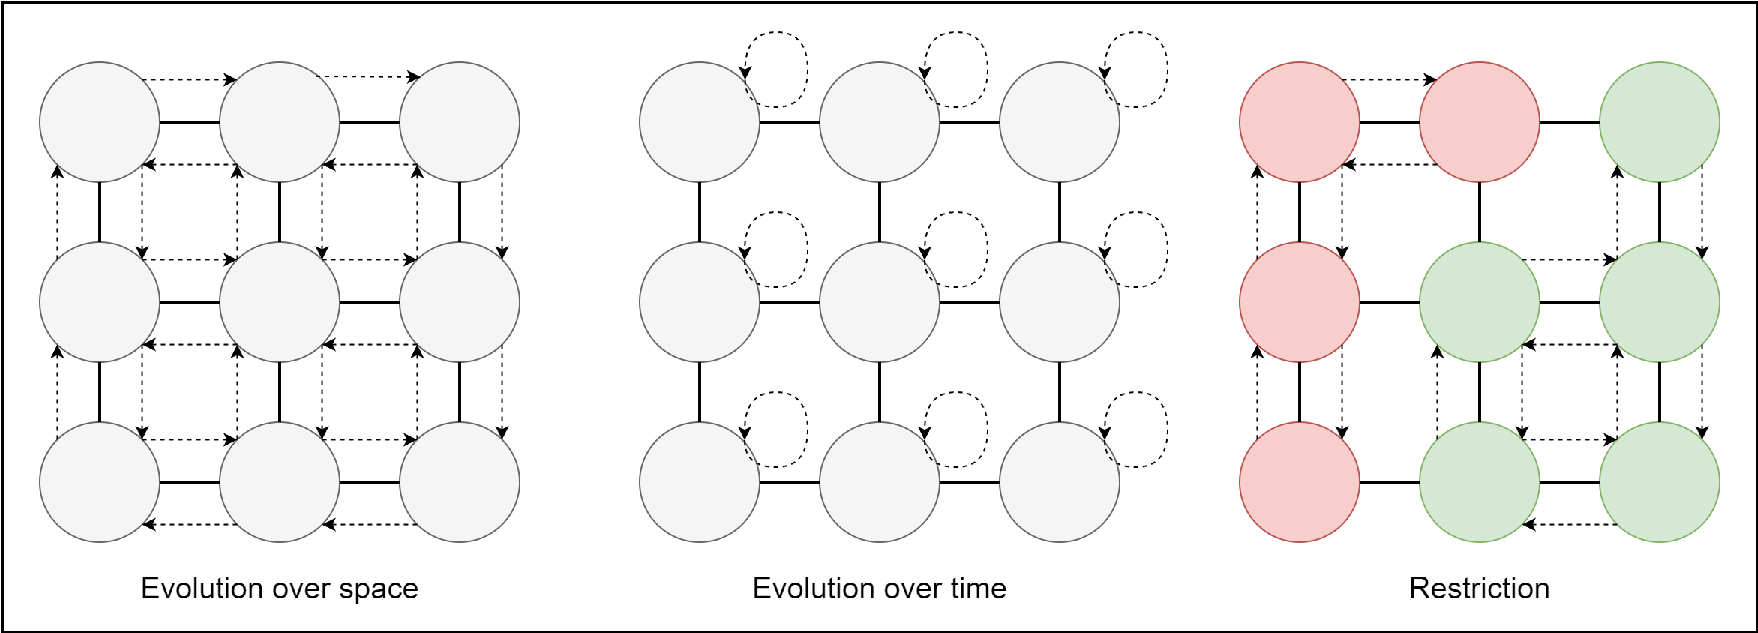
\includegraphics[width=1\textwidth]{resources/figures/information-propagation-in-field-calculus.pdf}
  \caption[Propagation of information in field calculus]{
    The three methods of propagation of information in field calculus. The figure
    shows three aggregates, each containing nine devices (\textit{circles}),
    connected by neighboring relations (\textit{solid lines}). Each
    aggregate shows the propagation of information (\textit{dashed arrows})
    using one of the methods of field calculus. Composition of these methods
    is also possible.
  }
  \label{figure:information-propagation-in-field-calculus}
\end{figure}

The evolution of a computational field refers to its gradual transformation
along the spatial or temporal dimensions. Evolution over space can be achieved
with \textit{inter-device communication}, including accumulation and
elaboration of neighboring events for producing the next event of each device.
Evolution over time can be obtained by specifying dependencies between the next
and previous events of each device (potentially an expression of
\textit{intra-device communication} or \textit{self-communication}).

The restriction of a computational field refers to the application of a
constraint on its evolution over space. Restriction can be achieved through
\textit{conditional partitioning of the network}, that is assigning each device
to a different partition depending on a given condition, such that neighbors
belonging to different partitions are isolated and cannot communicate despite
their neighboring relation. However, only the restricted computational field is
affected by the network partitions, so the information of other computational
fields may still propagate between partitions.

More formally, a program specification in field calculus can be written using
the abstract syntax in Figure \ref{figure:field-calculus-language}. One such
specification can be interpreted both at the \textit{macro-level} (as a
composition of collective operations on computational fields) and at the
\textit{micro-level} (as a composition of individual operations executed by
every device to compute and propagate its next event). Such equivalent
interpretations bridge the gap between the collective behavior of the aggregate
and the individual behaviors of its components.

\begin{figure}[!ht]
  \centering
  \noindent\setlength{\fboxsep}{0pt}\fbox{
    \begin{minipage}{0.95\textwidth}
      \begin{align*}
        P \quad\Rightarrow\quad    & F^*e                                 & \textit{Program}              &                                                      \\
        F \quad\Rightarrow\quad    & \texttt{def } d(x^*)\{e\}            & \textit{Function Declaration} &                                                      \\
        e \quad\Rightarrow\quad    & x                                    & \textit{Expression}           & : \textit{Variable}                                  \\
        \quad|\quad                & v                                    &                               & : \textit{Value}                                     \\
        \quad|\quad                & f(e^*)                               &                               & : \textit{Function Call}                             \\
        \quad|\quad                & \texttt{nbr}\{e\}                    &                               & : \textit{Evolution over space}                      \\
        \quad|\quad                & \texttt{rep}(e)\{(x) \rightarrow e\} &                               & : \textit{Evolution over time}                       \\
        \quad|\quad                & \texttt{if}(e)\{e\}\{e\}             &                               & : \textit{Restriction}                               \\
        f \quad\Rightarrow\quad    & d                                    & \textit{Function Name}        & : \textit{User-declared}                             \\
        \quad|\quad                & b                                    &                               & : \textit{Built-in}                                  \\
        v \quad\Rightarrow\quad    & l                                    & \textit{Value}                & : \textit{Local Value}                               \\
        \quad|\quad                & \phi                                 &                               & : \textit{Neighbouring Value}                        \\
        l \quad\Rightarrow\quad    & \texttt{c}(l^*)                      & \textit{Local Value}          & : \textit{Constructor Call}                          \\
        \phi \quad\Rightarrow\quad & \delta^* \rightarrow l^*             & \textit{Neighbouring Value}   & : \textit{Devices} \rightarrow \textit{Local Values} \\
      \end{align*}
    \end{minipage}
  }
  \caption[An abstract syntax for field calculus]{
  An abstract syntax for field calculus \cite{FieldCalculus-AggregateComputing}.
  The symbol $a^*$ indicates a possibly empty sequence of $a$ (e.g.,
  $a_1,...,a_n$ with $n \geq 0$), while the symbol $a^*{\rightarrow}b^*$ a
  possibly empty sequence of relations $a_1{\rightarrow}b_1,...,a_n{\rightarrow}b_n$.
  On the left, the production rules of the language. On the right, the
  meaning of the left and right side of each production rule.
  }
  \label{figure:field-calculus-language}
\end{figure}

A \textbf{program} is a sequence of \textbf{function declarations} followed by
an \textbf{expression}, which determines the behavior of the system. An
expression can be:
\begin{itemize}
  \item A \textbf{variable}, referencing information (e.g., a function
        parameter).
  \item A \textbf{value}, expressing information. A value can be either a
        \textbf{local value} (e.g., a boolean, a number, any object) or a
        \textbf{neighboring value}, which is a function mapping, for each
        device, the neighbors to a local value.
  \item A \textbf{function call}, describing the composition of computational
        fields. The called function can be either \textbf{user defined} (i.e.,
        referencing a function declaration) or \textbf{built-in} (e.g.,
        arithmetic or logical operators).
  \item A \textbf{communication expression} $\texttt{nbr}\{e\}$, describing the
        evolution over space of a computational field. In detail, the
        expression yields a neighboring value computed in two steps: first,
        each device computes the expression $e$, sharing the result with its
        neighbors; then, each device collects the results of its neighbors,
        producing a neighboring value of the latest evaluation of $e$.
  \item An \textbf{iteration expression} $\texttt{rep}(e_1)\{(x) \rightarrow
        e_2 \}$, describing the evolution over time of a computational field.
        In detail, the expression is computed iteratively, each iteration
        yielding a result $v_i$, with $i$ being the number of iterations
        computed so far. The result $v_0$ computed in the first iteration is
        the value yielded by $e_1$, while successive results $v_k$ ($k > 0$)
        are computed in the following iterations as the value yielded by $e_2$
        when applying the function $s: (x) \rightarrow e_2$ to the result
        $v_{k-1}$ of the previous iteration ($v_k = s(v_{k-1})$).
  \item A \textbf{branching expression} $\texttt{if}(e_1)\{e_2\}\{e_3\}$,
        describing the restriction of a computational field. In detail, the
        computation in the system is split depending on the condition $e_1$
        (i.e., an expression evaluating to either true or false), resulting in
        the computation of ${e_2}$ where and when $e_1$ is satisfied or in the
        computation of $e_3$ otherwise.

        In the branching expression, restriction happens as a consequence of
        \textbf{alignment}. Alignment is the process of keeping track of the
        structure of a specification (e.g., using an abstract syntax tree), in
        order to ensure correct message matching during communication when the
        specification contains different instances of \texttt{nbr} or
        \texttt{rep} constructs. Due to alignment, communication between a
        device and a neighbor can only happen if they are computing two
        expressions that share a \texttt{nbr} construct in the same position
        within the structure of the program. In particular, within the
        branching expression, alignment forbids communication between devices
        computing $e_2$ and $e_3$, as these expressions belong to two different
        branches of the program specification.
\end{itemize}

While field calculus provides solutions for the composition and evolution of
global or regional behaviors in aggregates, its syntax is also too general for
it to be resilient and too succinct for programming to be simple. Aggregate
computing addresses the problems by implementing three \textit{resilient
higher-order primitives} on top of field calculus (Listing
\ref{listing:aggregate-computing-blocks} and Figure
\ref{figure:information-propagation-in-aggregate-computing}).

\begin{figure}[!ht]
  \lstinputlisting[
    caption={
        [The higher-order primitives of aggregate computing]
        The three higher-order primitives introduced by aggregate computing
        on top of field calculus.
      },
    captionpos=b,
    label={listing:aggregate-computing-blocks}
  ]{resources/listings/aggregate-computing-blocks.txt}
  \centering
  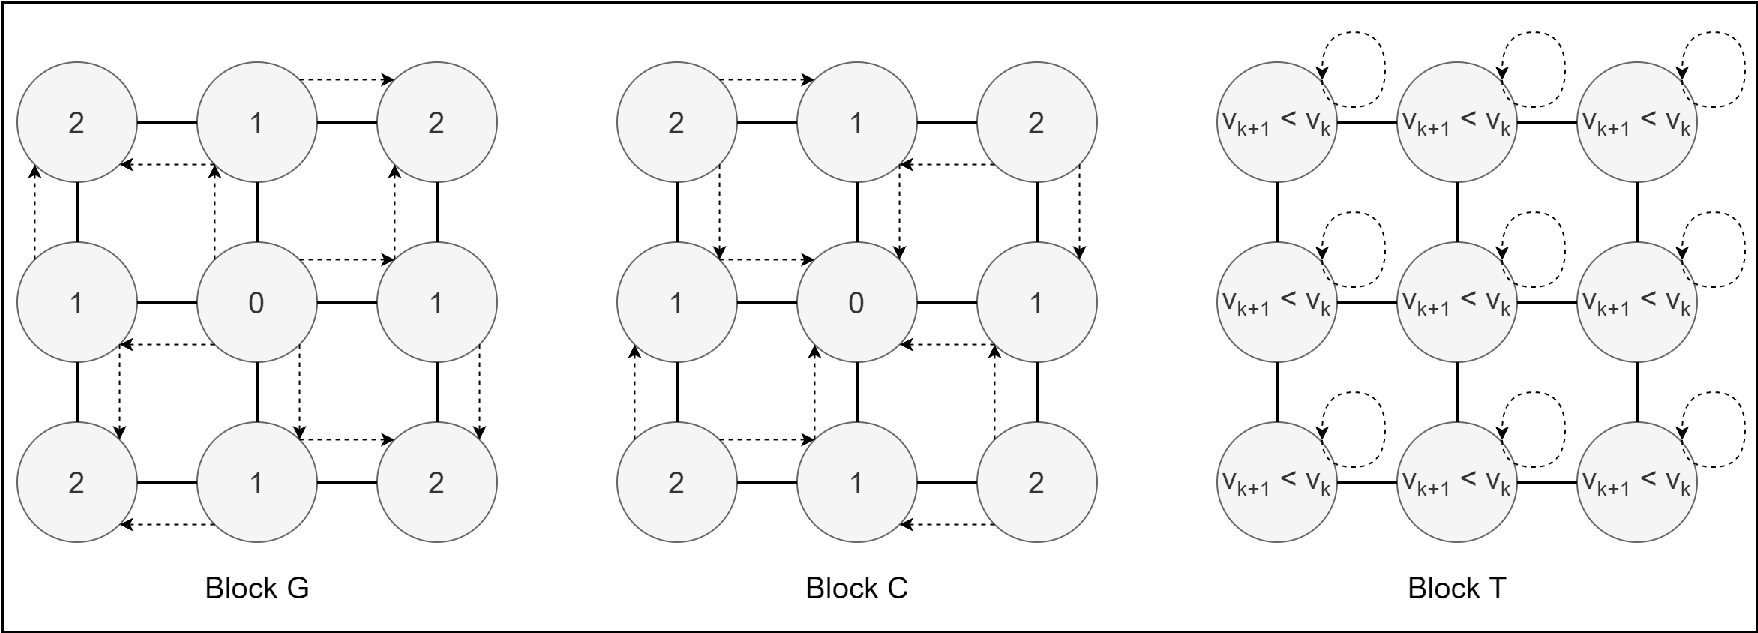
\includegraphics[width=1\textwidth]{resources/figures/information-propagation-in-aggregate-computing.pdf}
  \caption[Propagation of information in aggregate computing]{
    The three resilient methods of propagation of information in aggregate
    computing: \texttt{Block G} propagates information towards the direction of
    increasing gradient (\textit{value inside each device}), diffusing
    information; \texttt{Block C} propagates information towards the direction
    of decreasing gradient, collecting information; \texttt{Block T} evolves
    information in time, applying a decay until convergence to a minimum value.
    Note that the diagrams only shows \textit{relevant} propagation of
    information, hiding the underlying communication required to attain such
    behavior.
  }
  \label{figure:information-propagation-in-aggregate-computing}
\end{figure}

The \texttt{Block G} primitive \cite{CAS-AggregateComputingBlocks} handles the
diffusion of information by computing the \textbf{gradient} (i.e., the
computational field of distances) with respect to a \texttt{source}, while
accumulating values towards the direction of increasing gradient. Accumulation
starts from an \texttt{initial} value at the \texttt{source} and proceeds
hop-by-hop using an \texttt{accumulator} moving away from the \texttt{source}.
The distance between a device and its neighbors (used for computing the
gradient) is defined by a \texttt{metric}.

The \texttt{Block C} primitive handles the convergence of information, using a
\texttt{potent\-ial} (e.g., a gradient) to accumulate values towards the
direction of decreasing \texttt{potent\-ial}. In this sense, the \texttt{Block
C} primitive is complementary to the \texttt{Block G} primitive. Accumulation
proceeds with each device applying an \texttt{accumulator} to a \texttt{null}
value (idempotent for the \texttt{accumulator}), its \texttt{local} value and
the values of any neighbor with a higher \texttt{potential}.

Finally, the \texttt{Block T} primitive handles the evolution of information in
time, starting from an \texttt{initial} maximum value for each device and
reducing it at each computation round using a \texttt{decay} function, until a
\texttt{final} minimum value is reached.

These aggregate computing primitives cover the most common applications when
programming aggregates, while offering additional resilience compared to field
calculus due to their \textbf{self-stabilization} property, which guarantees
convergence towards a final stable state for the aggregate after some time
without changes in its environment or its network topology. As such, they can
be used as building blocks in \textit{general or domain-specific libraries} for
aggregate computing (e.g., swarm coordination framework \cite{MacroSwarm}),
increasingly reducing the complexity of programming aggregates of devices.